% Feb10 -- Addresses review/requests


%%====================================================================== change
% University of Waterloo Thesis Template for LaTeX
% Last Updated August 21, 2018
% by Stephen Carr, IST Client Services, git
% University of Waterloo, 200 University Ave. W., Waterloo, Ontario, Canada
% FOR ASSISTANCE, please send mail to rt-IST-CSmathsci@rt.uwaterloo.ca

% DISCLAIMER
% To the best of our knowledge, this template satisfies the current uWaterloo thesis requirements.
% However, it is your responsibility to assure that you have met all
% requirements of the University and your particular department.

% Many thanks for the feedback from many graduates who assisted the development of this template.
% Also note that there are explanatory comments and tips throughout this template.
%======================================================================
% Some important notes on using this template and making it your own...

% The University of Waterloo has required electronic thesis submission since October 2006.
% See the uWaterloo thesis regulations at
% https://uwaterloo.ca/graduate-studies/thesis.
% This thesis template is geared towards generating a PDF
% version optimized for viewing on an electronic display, including
% hyperlinks within the PDF.

% DON'T FORGET TO ADD YOUR OWN NAME AND TITLE in the "hyperref" package
% configuration below. THIS INFORMATION GETS EMBEDDED IN THE PDF FINAL PDF DOCUMENT.
% You can view the information if you view properties of the PDF document.

% Many faculties/departments also require one or more printed
% copies. This template attempts to satisfy both types of output. See additional notes below.
% It is based on the standard "book" document class which provides all necessary
% sectioning structures and allows multi-part theses.

% If you are using this template in Overleaf (cloud-based collaboration service), then it is
% automatically processed and previewed for you as you edit.

% For people who prefer to install their own LaTeX distributions on their own computers, and process
% the source files manually, the following notes provide the sequence of tasks:

% E.g. to process a thesis called "mythesis.tex" based on this template, run:

% pdflatex mythesis	-- first pass of the pdflatex processor
% bibtex mythesis	-- generates bibliography from .bib data file(s)
% makeindex         -- should be run only if an index is used
% pdflatex mythesis	-- fixes numbering in cross-references, bibliographic references, glossaries, index, etc.
% pdflatex mythesis	-- it takes a couple of passes to completely process all cross-references

% If you use the recommended LaTeX editor, Texmaker, you would open the mythesis.tex
% file, then click the PDFLaTeX button. Then run BibTeX (under the Tools menu).
% Then click the PDFLaTeX button two more times. If you have an index as well,
% you'll need to run MakeIndex from the Tools menu as well, before running pdflatex
% the last two times.

% N.B. The "pdftex" program allows graphics in the following formats to be
% included with the "\includegraphics" command: PNG, PDF, JPEG, TIFF
% Tip 1: Generate your figures and photos in the size you want them to appear
% in your thesis, rather than scaling them with \includegraphics options.
% Tip 2: Any drawings you do should be in scalable vector graphic formats:
% SVG, PNG, WMF, EPS and then converted to PNG or PDF, so they are scalable in
% the final PDF as well.
% Tip 3: Photographs should be cropped and compressed so as not to be too large.

% To create a PDF output that is optimized for double-sided printing:
%
% 1) comment-out the \documentclass statement in the preamble below, and
% un-comment the second \documentclass line.
%
% 2) change the value assigned below to the boolean variable
% "PrintVersion" from "false" to "true".

%======================================================================
%   D O C U M E N T   P R E A M B L E
% Specify the document class, default style attributes, and page dimensions, etc.
% For hyperlinked PDF, suitable for viewing on a computer, use this:
\documentclass[letterpaper,12pt,titlepage,oneside,final]{book}

% For PDF, suitable for double-sided printing, change the PrintVersion variable below
% to "true" and use this \documentclass line instead of the one above:
%\documentclass[letterpaper,12pt,titlepage,openright,twoside,final]{book}

% Some LaTeX commands I define for my own nomenclature.
% If you have to, it's easier to make changes to nomenclature once here than in a
% million places throughout your thesis!
\newcommand{\package}[1]{\textbf{#1}} % package names in bold text
\newcommand{\cmmd}[1]{\textbackslash\texttt{#1}} % command name in tt font
% print-optimized version will ignore \href tags (redefined by hyperref pkg).
%\newcommand{\texorpdfstring}[2]{#1} % does nothing, but defines the command
% Anything defined here may be redefined by packages added below...

% This package allows if-then-else control structures.
\usepackage{ifthen}
\usepackage{comment}
\usepackage{tikz}
%% -------------------------------------- Declare the layers
\pgfdeclarelayer{nodelayer}
\pgfdeclarelayer{edgelayer}
\pgfsetlayers{edgelayer,nodelayer,main}

%% -------------------------------------- Declare the styles
% Node styles
\tikzstyle{new style 0}=[fill=white, draw=black, shape=circle]
\tikzstyle{invisibox}=[fill=white, draw=white, shape=rectangle]
\tikzstyle{cir}=[fill=white, draw=white, shape=circle]

% Edge styles
\tikzstyle{larrow}=[<-]
\usepackage{amsthm}
\usepackage{tikz-cd}
\usepackage{caption}
\usepackage{subfig}
\usepackage{svg}
\usepackage{listings}
\usepackage[titletoc]{appendix}% https://ctan.org/pkg/appendix
\documentclass{report}
\newboolean{PrintVersion}
\setboolean{PrintVersion}{false}
% CHANGE THIS VALUE TO "true" as necessary, to improve printed results for hard copies
% by overriding some options of the hyperref package, called below.
\renewcommand\lstlistingname{Listing}
\renewcommand\lstlistlistingname{List of Listings}


%\usepackage{nomencl} % For a nomenclature (optional; available from ctan.org)
\usepackage{amsmath,amssymb,amstext} % Lots of math symbols and environments

\newcommand{\floor}[1]{\left\lfloor #1 \right\rfloor}
\newcommand{\ceil}[1]{\left\lceil #1 \right\rceil}

\usepackage{mdframed,lipsum}

\newtheorem{conjecture}{Conjecture}
\newtheorem{definition}{Definition}
\newtheorem{theorem}{Theorem}
\newtheorem{proposition}{Proposition}
\newtheorem{lemma}{Lemma}
\makeatletter
\renewcommand*\env@matrix[1][*\c@MaxMatrixCols c]{%
\hskip -\arraycolsep
\let\@ifnextchar\new@ifnextchar
\array{#1}}
\makeatother
% Hyperlinks make it very easy to navigate an electronic document.
% In addition, this is where you should specify the thesis title
% and author as they appear in the properties of the PDF document.
% Use the "hyperref" package
% N.B. HYPERREF MUST BE THE LAST PACKAGE LOADED; ADD ADDITIONAL PKGS ABOVE
\usepackage[pdftex,pagebackref=false]{hyperref} % with basic options
%\usepackage[pdftex,pagebackref=true]{hyperref}
% N.B. pagebackref=true provides links back from the References to the body text. This can cause trouble for printing.
\hypersetup{
plainpages=false,       % needed if Roman numbers in frontpages
unicode=false,          % non-Latin characters in Acrobat’s bookmarks
pdftoolbar=true,        % show Acrobat’s toolbar?
pdfmenubar=true,        % show Acrobat’s menu?
pdffitwindow=false,     % window fit to page when opened
pdfstartview={FitH},    % fits the width of the page to the window
%    pdftitle={uWaterloo\ LaTeX\ Thesis\ Template},    % title: CHANGE THIS TEXT!
%    pdfauthor={Author},    % author: CHANGE THIS TEXT! and uncomment this line
%    pdfsubject={Subject},  % subject: CHANGE THIS TEXT! and uncomment this line
%    pdfkeywords={keyword1} {key2} {key3}, % list of keywords, and uncomment this line if desired
pdfnewwindow=true,      % links in new window
colorlinks=true,        % false: boxed links; true: colored links
linkcolor=blue,         % color of internal links
citecolor=green,        % color of links to bibliography
filecolor=magenta,      % color of file links
urlcolor=cyan           % color of external links
}
\ifthenelse{\boolean{PrintVersion}}{   % for improved print quality, change some hyperref options
\hypersetup{    % override some previously defined hyperref options
%    colorlinks,%
citecolor=black,%
filecolor=black,%
linkcolor=black,%
urlcolor=black}
}{} % end of ifthenelse (no else)

\usepackage{amsfonts}
\usepackage{bm}
\usepackage{graphicx} % Exception to the rule of hyperref being the last add-on package
% If glossaries-extra is not in your LaTeX distribution, get it from CTAN (http://ctan.org/pkg/glossaries-extra),
% although it's supposed to be in both the TeX Live and MikTeX distributions. There are also documentation and
% installation instructions there.
\usepackage{multirow}
\usepackage{color}
% Setting up the page margins...
% uWaterloo thesis requirements specify a minimum of 1 inch (72pt) margin at the
% top, bottom, and outside page edges and a 1.125 in. (81pt) gutter
% margin (on binding side). While this is not an issue for electronic
% viewing, a PDF may be printed, and so we have the same page layout for
% both printed and electronic versions, we leave the gutter margin in.
% Set margins to minimum permitted by uWaterloo thesis regulations:
\setlength{\marginparwidth}{0pt} % width of margin notes
% N.B. If margin notes are used, you must adjust \textwidth, \marginparwidth
% and \marginparsep so that the space left between the margin notes and page
% edge is less than 15 mm (0.6 in.)
\setlength{\marginparsep}{0pt} % width of space between body text and margin notes
\setlength{\evensidemargin}{0.125in} % Adds 1/8 in. to binding side of all
% even-numbered pages when the "twoside" printing option is selected
\setlength{\oddsidemargin}{0.125in} % Adds 1/8 in. to the left of all pages
% when "oneside" printing is selected, and to the left of all odd-numbered
% pages when "twoside" printing is selected
\setlength{\textwidth}{6.375in} % assuming US letter paper (8.5 in. x 11 in.) and
% side margins as above
\raggedbottom

% The following statement specifies the amount of space between
% paragraphs. Other reasonable specifications are \bigskipamount and \smallskipamount.
\setlength{\parskip}{\medskipamount}

% The following statement controls the line spacing.  The default
% spacing corresponds to good typographic conventions and only slight
% changes (e.g., perhaps "1.2"), if any, should be made.
\renewcommand{\baselinestretch}{1} % this is the default line space setting


% By default, each chapter will start on a recto (right-hand side)
% page.  We also force each section of the front pages to start on
% a recto page by inserting \cleardoublepage commands.
% In many cases, this will require that the verso (left-hand) page be
% blank, and while it should be counted, a page number should not be
% printed.  The following statements ensure a page number is not
% printed on an otherwise blank verso page.
\let\origdoublepage\cleardoublepage
\newcommand{\clearemptydoublepage}{%
\clearpage{\pagestyle{empty}\origdoublepage}}
\let\cleardoublepage\clearemptydoublepage

% Define Glossary terms (This is properly done here, in the preamble and could also be \input{} from a separate file...)
%% Main glossary entries -- definitions of relevant terminology
%\newglossaryentry{computer}
%{
%name=computer,
%description={A programmable machine that receives input data,
%stores and manipulates the data, and provides
%formatted output}
%}

% Nomenclature glossary entries -- New definitions, or unusual terminology
%\newglossary*{nomenclature}{Nomenclature}
%\newglossaryentry{dingledorf}
%{
%type=nomenclature,
%name=dingledorf,
%description={A person of supposed average intelligence who makes incredibly brainless misjudgments}
%}

% List of Abbreviations (abbreviations type is built in to the glossaries-extra package)
%\newabbreviation{aaaaz}{AAAAZ}{American Association of Amateur Astronomers and Zoologists}
%
%% List of Symbols
%\newglossary*{symbols}{List of Symbols}
%\newglossaryentry{rvec}
%{
%name={$\mathbf{v}$},
%sort={label},
%type=symbols,
%description={Random vector: a location in n-dimensional Cartesian space, where each dimensional component is determined by a random process}
%}
%\lstset{basicstyle=\ttfamily}
%\makeglossaries
\lstdefinestyle{mystyle}{
    commentstyle=\color{olive},
    keywordstyle=\color{magenta},
    numberstyle=\tiny\color{gray},
    stringstyle=\color{violet},
    basicstyle=\ttfamily\footnotesize,
    breakatwhitespace=false,
    breaklines=true,
    captionpos=b,
    keepspaces=true,
    numbers=left,
    numbersep=5pt,
    showspaces=false,
    showstringspaces=false,
    showtabs=false,
    tabsize=2
}

\renewcommand{\cftchappresnum}{\normalfont}


%======================================================================
%   L O G I C A L    D O C U M E N T
% The logical document contains the main content of your thesis.
% Being a large document, it is a good idea to divide your thesis
% into several files, each one containing one chapter or other significant
% chunk of content, so you can easily shuffle things around later if desired.
%======================================================================
\begin{document}

%----------------------------------------------------------------------
% FRONT MATERIAL
% title page,declaration, borrowers' page, abstract, acknowledgements,
% dedication, table of contents, list of tables, list of figures, nomenclature, etc.
%----------------------------------------------------------------------
    % T I T L E   P A G E
% -------------------
% Last updated June 14, 2017, by Stephen Carr, IST-Client Services
% The title page is counted as page `i' but we need to suppress the
% page number. Also, we don't want any headers or footers.
\pagestyle{empty}
\pagenumbering{roman}


% The contents of the title page are specified in the "titlepage"
% environment.
\begin{titlepage}
    \begin{center}
        \vspace*{1.0cm}

        \Huge Mean Field Behaviour of Job Redundancy Queueing Models

        \vspace*{1.0cm}

        \normalsize
        by \\

        \vspace*{1.0cm}

        \Large
        Aaron Janeiro Stone \\

        \vspace*{3.0cm}


    \end{center}
\end{titlepage}

% The rest of the front pages should contain no headers and be numbered using Roman numerals starting with `ii'
\pagestyle{plain}
\setcounter{page}{2}

\cleardoublepage % Ends the current page and causes all figures and tables that have so far appeared in the input to be printed.
% In a two-sided printing style, it also makes the next page a right-hand (odd-numbered) page, producing a blank page if necessary.


% D E C L A R A T I O N   P A G E


\bigskip

\noindent
I understand that my thesis may be made electronically available to the public.

\cleardoublepage

% A B S T R A C T
% ---------------

\begin{center}
    \textbf{Abstract}
\end{center}
Technological advancement in cloud computing has resulted in the viability of a new class of
routing algorithm, the so-called redundancy models which are able to replicate jobs for processing on different
servers. An asymptotic amount of queue-endowed servers could in this way employ their plentiful, otherwise
idle servers towards processing.
Research on the behaviour of such systems, however, has only conjectured
the asymptotic independence of queues (Gardner et al., 2017;
Hellemans et al., 2019).
To this end, by modelling the process as a time-indexed family of hypergraphs wherein
hyperedges represent cloned dependents,  along with the notion of exchangeable
random groups derived by Austin (2008), we are able to demonstrate the conjectured behaviour in a simulation setting.

\cleardoublepage

% A C K N O W L E D G E M E N T S
% -------------------------------

\begin{center}
    \textbf{Acknowledgements}
\end{center}
Thank you, Dr. Steve Drekic and Dr. Tim Hellemans, for your guidance as I delved into an area once foreign to me.

\cleardoublepage

% D E D I C A T I O N
% -------------------

\begin{center}
    \textbf{Dedication}
\end{center}

Thank you, Fatima and my family, for always being there for me in such a fast-moving world.

\quad

\textit{The whole entire world is a very narrow bridge; the main thing is to have no fear at all.}
\flushright - \textit{Nachman}
\flushleft
\cleardoublepage

% T A B L E   O F   C O N T E N T S
% ---------------------------------
\renewcommand\contentsname{Table of Contents}
\tableofcontents
\cleardoublepage
\phantomsection    % allows hyperref to link to the correct page

% L I S T   O F   T A B L E S
% ---------------------------
\addcontentsline{toc}{chapter}{List of Tables}
\listoftables
\cleardoublepage
\phantomsection		% allows hyperref to link to the correct page

% L I S T   O F   F I G U R E S
% -----------------------------
\addcontentsline{toc}{chapter}{List of Figures}
\listoffigures
\cleardoublepage
\phantomsection        % allows hyperref to link to the correct page

% L I S T  O F  L I S T I N G S
% -----------------------------
\addcontentsline{toc}{chapter}{List of Listings}
\lstlistoflistings
\cleardoublepage
\phantomsection        % allows hyperref to link to the correct page

% Change page numbering back to Arabic numerals
\pagenumbering{arabic}



%----------------------------------------------------------------------
% MAIN BODY
% We suggest using a separate file for each chapter of your thesis.
% Start each chapter file with the \chapter command.
% Only use \documentclass or \begin{document} and \end{document} commands
% in this master document.
% Tip 4: Putting each sentence on a new line is a way to simplify later editing.
%----------------------------------------------------------------------
%======================================================================


\chapter{Introduction}\label{ch:introduction2}\label{ch:introduction}
%======================================================================
Enamoured by physicists for its ability to turn probabilistic behaviour into matters of determinism, Mean Field Theory (MFT) also has a place in the study of queueing systems as the number of queues become asymptotic.
\begin{definition}[Mean Field]
    \hfill \\
    Over a time-filtered probability space $(\Omega, \mathcal{F}_{t},\mathcal{F},P)$, for $N \in \mathbb{N}$, a mean field describes the behaviour of any set of stochastic random variables
    \[
        \mathbf{X}^{(N)}(t) := \{X_{i}(t)\}_{i \leq N}
    \]
    that turns deterministic in law as $N \rightarrow \infty$, irrespective of if the finite-$N$ or finite-$t$ cases resulted in this set of bodies being dependent~\cite{mukhopadhyay_analysis_nodate}.
\end{definition}

Next, it is important to define exchangeability, a condition which provides useful properties for MFT.

\begin{definition}[Exchangeability]
    A collection of random variables $\mathbf{X}^{(N)}$ is exchangeable if for any $N$-permutation $\gamma_{N} \in \Gamma_{N}$, \[\text{Law}(\gamma_{N} \mathbf{X}^{(N)}) = \text{Law}( \mathbf{X}^{(N)}).\] de Finetti's Theorem states that exchangeability implies the collection to be conditionionally independent (in a Markovian sense) and identically distributed~\cite{austin_exchangeable_2015}.
    Moreover, for partition $N=\bigcup_{i \leq k}N_{i}$, exchangeability over partition $\{N_{i}\}_{i\leq k }$ such that
    \[
        \text{Law}(\mathbf{X}^{(\gamma\{N_{i}\}_{i\leq k })}) = \text{Law}(\mathbf{X}^{(\{N_{i}\}_{i\leq k })})
    \] is known as $(N,\Gamma)$ exchangeability (with $\gamma \in \Gamma$)~\cite{austin_exchangeable_2008}.
\end{definition}
With multiprocessing being employed at its current scale in server farms, society is indeed approaching a time wherein the asymptotic behaviour of parallel queueing systems can be considered realistically.
Lately, interest has been given to queueing systems which employ job redundancy in order to lower total processing time~\cite{ayesta_unifying_2018}.
That is, routing policies which take advantage of scenarios wherein a surplus of queues and/or servers are available, replicating each job such that it might be completed faster should it happen to make its way through a less-busy queue than the original.
\begin{definition}[Job Redundancy]
    \hfill \\
    A scheduler, $\mathcal{D}$, follows a job redundancy policy if it systematically clones arriving jobs and removes all clones upon (or after a delay following) completion of any one clone.
\end{definition}
Prior studies have pointed towards certain redundancy policies as being inefficient or even unrealistic due to over-relying on cloning.
Take for example \textit{Redundancy-d}, wherein $d$ servers are chosen per arrival;
each is given a clone and upon completion of any one clone, all others are removed immediately without any cost.
As such, implementing a threshold on when  to clone a job becomes useful for budgeting cancellation costs.
In particular, \textit{Threshold(R,d)} has risen to prominence as a means to balance workload in queueing systems.
\begin{definition}[Workload and System Load]
    \hfill \\
    \textbf{Workload} refers to the total amount of work remaining (in time) for a queue.
    In trivial cases not involving enqueued bodies potentially leaving, this would merely be the sum of individual jobs' service times. With $w^{(i)}_{j} (t)$ denoting the (random) service time of the $j$th job in queue $X_{i}$ at time $t$, the workload of a queue would be:
    \begin{align}
        W_{i}(t) = \sum_{j \leq \#X_{i}(t)}w^{(i)}_{j}(t)
    \end{align}
    for counting measure $\#$ which counts the jobs waiting in a queue at some particular time. \textbf{System Load} refers to the amount of work remaining in the entire system,
    \begin{align*}
        W(t) = \sum_{i \in \psi}W_{i}(t)
    \end{align*}
    where $\psi \subseteq \mathbb{N}$, given that we will be considering the case of systems operating in finite time as the number of queues grows indefinitely.
    As such, $\psi$ will henceforth refer to this more general case.
    As such, $\psi$ will henceforth refer to this more general case.
\end{definition}
As an example, a service time in a $G/M/c$ system will be drawn from an exponential distribution. In this simple case,
the $m$th arriving job can be given the ``marks'' $(T_{m}, S_{m})\equiv (T, S)_{m}$ where
$S_{m} \overset{IID}\sim \text{EXP}(\lambda)$ and $T_{m}$ is the time of arrival. Conditioning on the process
$(T,S)_{m}$, $W_{i}(t)$ turns into a matter of merely adding up the enqueued service times and that remaining of the
currently serviced job, which is conveniently memoryless.

Altogether, Figure~\ref{fig:1} describes the behaviour which would be expected in an ideal system wherein both a mean field and asymptotic independence can be achieved~\cite{mukhopadhyay_analysis_nodate}. In particular, $P$ describes a fixed ``equilibrium'' point of the system,
a state of the system (in terms of queue-counts) which is consistently held once reached, giving the collection a distribution of $\delta_{P}$.
In terms of the predictability and stability of a system, needless to say, this would be a ``gold-standard";
one would be interested in their ability to achieve such a system in practice.

\begin{figure}
    \centering
    %! suppress = EscapeAmpersand
    \begin{tikzcd}[sep=huge]
        \mathbf{X}^{(N)}(t)\arrow[r, "N \rightarrow \infty"]\arrow[d,"t \rightarrow \infty"]
        & \mathbf{X}(t)\arrow[d, "t \rightarrow \infty"] \\
        \mathbf{X}^{(N)}(\infty)\arrow[r, "N \rightarrow \infty"]
        & \mathbf{\mathbf{\pi}}
    \end{tikzcd}
    \caption{Commutativity of Limits}
    \label{fig:1}
\end{figure}

For the sake of brevity, the notation of $[n] := \{i \in \mathbb{N} | i \leq n\}$ will be used, along with the understanding of $\mathbf{X}^{[n]} \equiv \mathbf{X}^{(n)}$ for maximal element $n$.
Moreover, accepting this set-index notation, $\mathbf{X}^{\psi}$ will refer to the general case of $[n]$, given we will also consider $[n] \overset{n\rightarrow \infty}\longrightarrow \mathbb{N}$.

\begin{definition}[Threshold($R,d$)]
    \hfill \\
    \textbf{Threshold(R,d)}, denoted $\mathcal{D}_{THRESH(R,d),Z}$, selects $d$ queues upon a job arrival.
    Next:
    \begin{enumerate}
        \item For $i \leq d$ queues which have workload less than or equal to $R$, place copies in these $i$ queues.
        \item If $i=0$, place the original arrival in a queue from the $d$ chosen at random.
    \end{enumerate}
    $Z$ refers to any imposed job cancellation cost (e.g., an added temporary workload).
\end{definition}


One important question, however, is yet to be answered.
It is unknown whether or not there exists sufficient arrival rate or service rate parameters such that a mean field will be observed for particular values of $R$ or $d$ in the threshold model.
This leads us to the following conjecture for which this paper aims to prove.
\begin{conjecture}
    \hfill \\
    As $N \longrightarrow \infty$, the system $\mathcal{D}_{THRESH(R,d),Z}$ becomes $(\psi, \Gamma)$-exchangeable. As $t \longrightarrow \infty$, the system becomes deterministic.
    \label{conj}
\end{conjecture}


%Note, however, that in this research we focus on $Z\equiv0$, being the case of no cancellation cost. We denote the policy $\mathcal{D}_{THRESH(R,d),Z=0}= \mathcal{D}_{THRESH(R,d)}$ for brevity. As Mukhopadhyay (2015) summarizes, the process of proving a problem of form \ref{conj} amounts to the following:
%\begin{enumerate}
%    \item
%    Show that the empirical distribution,
%    \begin{align}
%        X^{(N)}(t) = \frac{1}{N}\sum_{k=1}^{N}\mathbbm{1}_{\{\text{servers in state } E\}}
%        \label{emp}
%    \end{align}
%    converges weakly as $N\longrightarrow \infty$ to some process $X(t)$.
%    \item $X(t)$ converges to a degenerate distribution $\pi$ as $t \longrightarrow \infty$
%    \item $X^{(N)}(t) \overset{t \longrightarrow \infty}{\longrightarrow} X^{(N)}(\infty)$ weakly.
%    \item $X^{(N)}(\infty) \overset{N \longrightarrow \infty}{\longrightarrow} \pi$ as defined before.
%\end{enumerate}
%
%
%\section{Model Specification}
%In modelling the problem, we draw influence from the state space studied in \cite{bramson_asymptotic_2012} which proves asymptotic independence in the case of no job replications.
%\begin{definition}[State Space Without Redundancy]
%    \hfill \\
%    For $X^{*}_{n}(t)$ corresponding to the $n$th queue out of $N$,
%    \[X_{n}^{*}(t)\in (\mathbb{N},(\mathbb{R}^{+})^{3}):=\mathcal{E}^{(N)}_{n,*}\]
%    \[X^{*}(t) \in \{\mathcal{E}^{(N)}_{n}\}_{n \leq N} := \mathcal{E}_{*}^{(N)}\]
%    Corresponding to
%    \begin{enumerate}
%        \item $z_{n}(t) \in \mathbb{N}$ for queue size
%        \item $ w_{n}(t) \in \mathbb{R}^{+}$ for workload
%        \item $\ell_{n}(t) \in \mathbb{R}^{+}$ amount of service time spent on job in server
%        \item $v_{n}(t) \in \mathbb{R}^{+}$ time remaining
%    \end{enumerate}
%    \label{old}
%\end{definition}
%It was also shown in \ref{bram} that the model considered in \ref{old} can be thought of as a Piecewise Deterministic Markov Chain (PDMP); a such that, between Markovian events (arrivals and departures), only deterministic changes occur.
%
%In order to modify the state space described in \ref{old} to model our problem, we must address an additional problem introduced by the fact that now the dependency structure between jobs is an element of the state space which changes stochastically. In order to do so, we introduce a stochastic graph to model changes in dependence.
%
%\begin{definition}[Job Dependency Graph: Finite Case]
%    \hfill \\
%    The \textbf{Job Dependency Graph}, $G_{t}=(V,E)_{t}$ is held constant between the events of arrivals and job completions, where an edge is drawn between two nodes if and only if they are job-dependent.
%
%    \begin{enumerate}
%        \item Movement in a queue requires \textit{appropriate} redrawing of graph.
%        \item $G_{t}$ is stochastic with law in $\text{Pr}(\Omega, \mathcal{F}_{t})$.
%        \item Maximal system queue size is bounded, $\sup_{n \in N}z_{n}(t):=\nu(t).$
%    \end{enumerate}
%    "Appropriate redrawing" in this case means
%    \begin{enumerate}
%        \item The graph is redrawn to reflect movement within each queue (moving due to job completions or arrivals).
%        \item $G_{t}$ can depend only on $G_{s}, s <t $ and other current values of $X^{*}_{t}$ (denote these other values $\tilde X^{*}_{t}$) and is such that \[P(G_{t}|\tilde X^{*}_{t}, \{G_{a}\}_{a \in S})=P(G_{t}|\tilde X^{*}_{t}, G_{\max(S)})\]
%        for any set $S$ such that $ S \subset [0,t)$.
%    \end{enumerate}
%    \label{dep1}
%\end{definition}
%
%To illustrate, consider \ref{gee} as a realization at some fixed time $t$. One can, of course, describe this graph using an adjacency matrix of any labelling. For our purposes, we will employ a labelling which will segment vertices conveniently.
%
%\begin{definition}[Job Dependency Matrix: Finite Case]
%    \hfill \\
%    The \textbf{Job Dependency Matrix} is an adjacency matrix (non-unique but one-to-one) for $G_{t}$. Specifically,
%    \begin{align}
%        \rho(t)\equiv \rho(G_{t})=
%        \left[  \enskip
%        \begin{matrix}[c|c|c|c]
%            B_{1,1}  & B_{1,2}  & \dots & B_{1,\nu}\\
%            \hline
%            \vdots & \vdots & \vdots &\vdots  \\
%            \hline
%            B_{\nu,1}  & B_{\nu,2} & \dots   & B_{\nu,\nu}\\
%        \end{matrix} \enskip \right]
%        \label{rho}
%    \end{align}
%    is a blocked matrix such that submatrix
%    \[B_{i,j}= [b_{q,m}]_{q,m \leq N} = \begin{cases}
%                                            1, \substack{\text{ queue } q \text{ in row } i \text{ is connected in } G_{t} \\ \text{ to queue } m \text{ in row } j}\\
%                                            0, \text{otherwise}
%    \end{cases}\]
%    where connections between jobs occur if and only if the completion of one job implies the removal of all other connected jobs from the system.
%    \label{jdf}
%\end{definition}
%
%\begin{figure}[htbp]
%    \centering
%    \includesvg[scale=.75]{grapho.svg}
%    \caption{Illustration of $G(t)$. Observe that the first row of vertices correspond to jobs currently being serviced.}
%    \label{gee}
%\end{figure}
%
%
%It is useful in modelling the problem at hand to construct this graph as an \textit{infinite graph}. That is, one could view the graph described in \ref{dep1} as an embedding into a larger graph by merely considering more queues or a larger maximal queue size at any finite time $t$, corresponding to the adding of an additional column or row of vertices, respectively. Building a metric on an infinite graph space simplifies the matter of quantifying convergence in terms of $N$ significantly because all possible finite embeddings can be expressed in the same space as $N\rightarrow \infty$. Thus, let us consider \[\mathbb{E}:= \{\text{locally finite graphs}\}\]
%\begin{definition}[State Space With Redundancy]
%    \hfill \\
%    For $X^{*}_{n}(t)$ corresponding to the $n$th queue out of $N$,
%    \[X_{n}^{*}(t)\in (\mathbb{N},(\mathbb{R}^{+})^{3},\rho(\mathbb{E})):=\mathcal{E}^{(N)}_{n}\]
%    \[X^{*}(t) \in \{\mathcal{E}^{(N)}_{n}\}_{n \leq N} := \mathcal{E}^{(N)}\]
%    Corresponding to
%    \begin{enumerate}
%        \item $z_{n}(t) \in \mathbb{N}$ for queue size
%        \item $ w_{n}(t) \in \mathbb{R}^{+}$ for workload
%        \item $\ell_{n}(t) \in \mathbb{R}^{+}$ amount of service time spent on job in server
%        \item $v_{n}(t) \in \mathbb{R}^{+}$ time remaining
%        \item $A \in \rho(\mathbb{E})$ is a representation of the graph.
%    \end{enumerate}
%    \label{def:spec}
%\end{definition}
%For any element of $\mathbb{E}$, $\rho$ can be described as in \label{mohar}\ref{mohar} (pg. 246). Specifically, take $G_{t} \in \mathbb{E}$ and consider $e_{k} = (\delta_{ik}| i \in \mathbb{N})$. Graph local finiteness guarantees that for any adjacency matrix $\rho(G_{t})$,  $\rho(G_{t})e_{k}\in\ell^{2}$. Thus, using the $\ell^{2}$ inner product, $\langle \rho(G_{t})e_{k},e_{i} \rangle:=\left(\rho(G_{t})\right)_{ik}$ can be used in order to define the equivalence relation of job dependence for each $i,k$ as in \ref{jdf}, granting a bijection.









    %======================================================================

\chapter{Model Specification}\label{ch:model-specification}

In order to model such a system, we incorporate the notation most frequently seen in the
study of palm calculus \cite{baccelli_elements_2003}. Most importantly, assuming we delegate a probability space $(\Omega, \mathcal{F}_{t}, \mathcal{F}, P)$ with the measurable flow $\{\theta_{t}\}$ which is $P/\theta_{t}$ invariant (i.e., Ergodic such that $\theta_{t}M = M \text{  for some } M \in \mathcal{F} \Rightarrow P(M) \in \{0,1\}$), then the arrival process $A$ can be associated with the flow.
In a system with Markovian arrivals, the counting measure associated with the flow would necessarily be Poisson;
other so-called counting processes wherein inter-arrivals are determined by random or even deterministic periods of time can be used. Inter-arrival times (for arrival $n$ occurring at $T_{n}$), regardless of the generating process, shall be denoted
\[\tau_{n} = T_{n+1}  - T_{n}, n \in \mathbb{N}.\]
Intensities (even if non-Poisson) will be denoted $\lambda = E(A((0,1])))$ for arrival process $A$, being interpreted as the intensity of a process moving a state (i.e., counting an additional element) within unit time.
\begin{definition}[Marked Process]
    For each job which enters the system, they can be ``marked" by a series of random variables defining their behaviour within the system \cite{baccelli_elements_2003}. In general, for the systems we shall consider, we consider the marked process $\sigma_{n}$ as being the required service of arrival $n$ and the marks $T_{n}$ as its time of arrival.
    The tuple \[(T,\sigma)_{n}, n \in \mathbb{N}\] will therefore be used to mark the $n$th job.
    We shall extend this notation, however, to include sets;
    for a set of jobs $\eta$, wherein each element has their own arrival time,
    \[(T, \sigma)_{\eta} = \{(T,\sigma)_{n}\}_{n \in \eta}.\]
\end{definition}

In a simple $G/M/c$ queue, as discussed before, the double $(T,\sigma)_{n}$ would be sufficient for reducing the problem into a deterministic one.
In our case, given that jobs can find their status in the system tied to the behaviour of their replicas, we must append a marking to track this phenomenon.
As a matter of fact, we instead move to marking the queues as was done by \cite{bramson_asymptotic_2012} to prove the conjecture in the case of Join-The-Shortest-Queue($d$) systems, although with an additional job dependency term.

\begin{definition}[Job Dependency Graph: Finite Case]
    \hfill \\
    The \textbf{Job Dependency Graph}, $G_{t}=(V,E)_{t}$, is held constant between the events of arrivals and job completions, where an edge is drawn between two nodes if and only if they are job-dependent. Moreover:

    \begin{enumerate}
        \item Movement in a queue requires \textit{appropriate} redrawing of graph.
        \item $G_{t}$ is stochastic with law in $\text{Pr}(\Omega, \mathcal{F}_{t})$.
        \item Maximal system queue size is bounded, $\sup_{n \in \chi}z_{n}(t):=\nu(t).$
    \end{enumerate}
    ``Appropriate redrawing" in this case means:
    \begin{enumerate}
        \item The graph is redrawn to reflect movement within each queue (moving due to job completions or arrivals).
        \item $G_{t}$ can depend only on $G_{s}, s <t$, and other current values of $X_{t}$ (denote these other values by $\tilde X_{t}$) and is such that \[P(G_{t}|\tilde X_{t}, \{G_{a}\}_{a \in S})=P(G_{t}|\tilde X_{t}, G_{\max(S)})\]
        for any set $S$ such that $ S \subset [0,t)$.
    \end{enumerate}
    \label{dep1}
\end{definition}
\begin{definition}[Job Dependency Matrix: Finite Case]
    \hfill \\
    The \textbf{Job Dependency Matrix} is an adjacency matrix (non-unique but one-to-one) for $G_{t}$. Specifically,
    \begin{align}
        \rho(t)\equiv \rho(G_{t})=
        \left[  \enskip
        \begin{matrix}[c|c|c|c]
            B_{1,1}  & B_{1,2}  & \dots & B_{1,\nu}\\
            \hline
            \vdots & \vdots & \vdots &\vdots  \\
            \hline
            B_{\nu,1}  & B_{\nu,2} & \dots   & B_{\nu,\nu}\\
        \end{matrix} \enskip \right]
        \label{rho}
    \end{align}
    is a blocked matrix such that sub matrix
    \[B_{i,j}= [b_{q,m}]_{q,m \leq N} = \begin{cases}
                                            1, \substack{if \text{ queue } q \text{ in row } i \text{ is connected in } G_{t} \\ \text{ to queue } m \text{ in row } j}\\
                                            0, \text{otherwise}
    \end{cases}\]
    where connections between jobs occur if and only if the completion of one job implies the removal of all other connected jobs from the system.
    \label{jdf}
\end{definition}

While complicated in the above form, this graph merely draws an edge between jobs of separate queues while tracking their current place in their respective queues. Because at most one event can happen in infinitesimal time (i.e., an arrival or departure), the assumptions merely state that between any two events this graph shall not need to be redrawn. Extending this notion, one can iterate such a procedure indefinitely, viewing the resultant infinite graph as one where jobs are joined by hyperedges if and only if there exists an element of a set of replicas in each of the queues. In other words, one can represent queues which are connected by means of having replicas of the same jobs enqueued within them by viewing each as a node connected with a hyperedge; we will call queues related by such a hyperedge members of a \textit{replica class} . Thus, Definition \ref{dep1} can be represented more succinctly in a hypergraph form, allowing one to represent the cavity process studied in \cite{Hellemans}.

\begin{definition}[Hypergraph Representation of the Dependency Matrix]
    \hfill \\
    By collapsing edges as jobs and vertices as servers, all connected subgraphs of $G_{t}$ can be thought of as incident nodes with edges $i_{1}, \dots i_{j}$ for $j<d$, representing connected jobs. This gives us now only as many nodes as there are currently servers. Such a representation for $G_{t}$ will be denoted by $\mathcal{G}_{t}$. See Figure~\ref{fig:hyper} for a visual representation.
\end{definition}

\begin{figure}
    \centering
    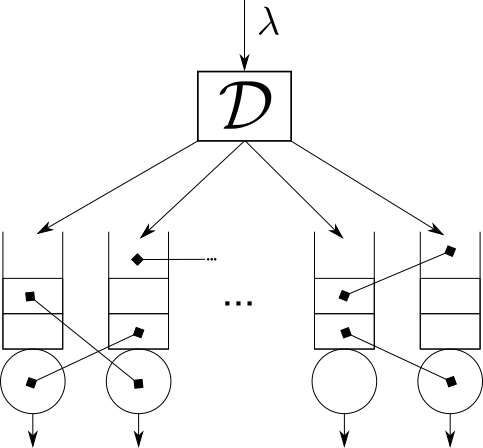
\includegraphics[scale=0.5]{systemredun}
    \caption{A graphical representation of queues with replicated jobs as hyperedges.}
    \label{fig:hyper}
\end{figure}

When one creates the infinite graph iteratively, it is meant that one could view the graph described in Definition \ref{dep1} as an embedding into a larger graph by merely considering more queues or a larger maximal queue size at any finite time $t$, corresponding to the adding of an additional column or row of vertices, respectively. Building a metric on an infinite graph space simplifies the matter of quantifying convergence in terms of $N$ significantly because all possible finite embeddings can be expressed in the same space as $N\rightarrow \infty$. Thus, let us consider \[\mathbb{E}:= \{\text{locally finite graphs}\}.\] Now, extending the notation of \cite{bramson_asymptotic_2012}, we can fully describe the marked process for queues with general service times.
\begin{definition}[State Space With Redundancy]
    \hfill \\
    With $\psi$ as $[n]$ or $\mathbb{N}$, $\rho(\cdot)$ denoting the matrix representation of a graph, and $\mathbf{X}^{\psi}$ denoting a system of $\psi$ parallel queues,
    let us assign $X_{n}(t)$ to the $n$th queue of the $\psi$-indexed possible queues such that $X_{n}(t)$ follows the $n$th marginal distribution of $\mathbf{X}^{\psi}$.
    Adapting the notation of \cite{bramson_asymptotic_2012}, we assign state spaces to $X_{n}$ and $\mathbf{X}^{\psi}$ as follows:
        \[X_{n}(t)\in (\mathbb{N},\left(\mathbb{R}^{+}\right)^{3},\rho(\mathbb{E})):=\mathcal{E}^{(\psi)}_{n}\]
    and
        \[\mathbf{X}(t) \in \{\mathcal{E}^{(\psi)}_{n}\}_{n \in \psi} := \mathcal{E}^{(\psi)},\]
    such that $X_{n} = (z_{n}(t), w_{n}(t),l_{n}(t),v_{n}(t),A(t))$ where
    \begin{enumerate}
        \item $z_{n}(t) \in \mathbb{N}$ denotes queue size,
        \item $ w_{n}(t) \in \mathbb{R}^{+}$ denotes workload,
        \item $\ell_{n}(t) \in \mathbb{R}^{+}$ denotes the amount of service time spent on job currently with server,
        \item $v_{n}(t) \in \mathbb{R}^{+}$ denotes the time remaining for job in server,
        \item $A \in \rho(\mathbb{E})$ is a representation of the graph,
    \end{enumerate}
    \label{def:spec}
\end{definition}


%======================================================================
%\begin{definition}(Hypergraph Representation of the Dependency Matrix)
%By collapsing edges as jobs and vertices as servers, all connected subgraphs of $G_{t}$ can be thought of as incident nodes with edges ${i_{1}, \dots, i_{j}}_{j<d}$ representing connected jobs. This gives us now only as many nodes as there are currently servers.
%\end{definition}
%
%Following with \cite{newgraph} for the remainder of the paper, the following assumption is made (and indeed can always be constructed):
%$G_{t}$ has the rooted graph component $(G_{t},o)$ for $o \in E(G_{t})$ being an arbitrary, particular element. We call $[G_{t},o]$ the class of graphs root-isomorphic (that is, isomorphic with respect to the root) to $(G_{t},o)$.  Also define $G_{t}^{*}$ to be the class of rooted locally finite graphs on $G_{t}$. Define the metric $\alpha := \sup \{r \in \mathbb{N}| r = \text{minimum length of paths connecting two graphs' roots}\}$ and $d = \frac{1}{1+\alpha}$ as another; both exist on $G^{*}_{t}$ and it can be shown that $G^{*}$ is seperable and complete \ref{newgraph}. $U(G)$ defines the distribution on $G^{*}$ obtained by choosing a random vertex as a root. Lastly, $[N]$ will be used to denote a vertex set for a graph $G_{t}^{N}\in(G_{t}^{N})_{N \in \mathbb{N}}$.
%
%\begin{definition}(Spectral Measure, \cite{hualiue2015})
%\[\mu_{G, o}(A)=\frac{1}{\theta_{o}}\left\langle P_{A} \delta_{o}, \delta_{o}\right\rangle, \quad \forall A \subset[0,2].\]
%\end{definition}
%One can show that this generalizes the usual spectral measure on finite graphs. We now can introduce a relevant graph pseudo-metric.
%\begin{definition}(Wasserstein Mean Distance)
%With the usual Wasserstein distance being defined as \[d_{p}^{W}(\mu, v):=\left(\inf _{\pi \in \Pi(\mu, v)} \int_{| 0,2] \times | 0,2\}} d(x, y)^{p} d \pi(x, y)\right)^{1 / p}\] for $\pi$ being a measure of the joint distribution, the distance taken over the expectation of each measure is the Wasserstein Mean Distance.
%\end{definition}
%
%The prior definitions are required in order to be able to quantify convergence; the remainder of the paper shall concern detailing how this is achieved. Following Bramson (2012), a modification allows us a means to prove convergence through coupling. In our case, we merely need to only choose an initial condition where a workload-based loss function is minimized.
%
% \begin{definition}[\textit{Queued Loss}]
% \\~\\
% \[W^{(l)}_{n}:= \sum_{i\in[F]}\min_{j\in [J]}(V_{j_{i}}),\]
% Where $l$ denotes the index in the coupling, $[a]=\{1, \dots, a \}$, $V_{a}$ denotes the time (workload) that the $a$th job has remaining for processing, $F$ denotes the size of queue $n$, and $J$ is the number of copied jobs in the system for the $i$th job in the queue.
% \end{definition}
% \begin{definition}[\textit{Queued Loss Domination}]
% \\~\\
%$W^{(2)}$ is said to dominate $W^{(2)}$ in queued loss at time $t\in [\tau_{i}, \tau_{i+1})$, where $\tau_{i}$ is the $i$th arrival,if
%\[\sup_{A \in [\mathcal{F}_{\tau_{i}},\mathcal{F}_{\tau_{i+1}}),n \in [N]}W^{(1)}_{n} \leq \inf_{A \in [\mathcal{F}_{\tau_{i}},\mathcal{F}_{\tau_{i+1}}),n \in [N]}W^{(2)}_{n}.\]
%In the above case, we take $W^{(l)}_{n}\equiv W^{(l)}_{n}(A)$ as in the usual measure-theoretic definition of a random variable. We denote the case where the above holds true with the partial ordering $W^{(2)}\succ W^{(1)}$.
% \end{definition}
% An important result which follows is a connection to job-independent case.
% \begin{theorem}
% \[\sup_{A \in [\mathcal{F}_{\tau_{i}},\mathcal{F}_{\tau_{i+1}})}W^{(l)}_{n}=W_{n}^{(l)}|_{J=1}.\]
% \end{theorem}
% The above proposition is actually trivial given that between Markov arrivals and without any connections, the system behaves in the usual PDMP manner on workload, decreasing linearly. If one were to add a connection, however, should that connected job reach the server in its corresponding queue while in queue $n$ it waits, $W_{n}^{(l)}$ will decrease faster but cannot ever increase (until an arrival). This gives us the smallest possible value for the queued loss of system 2.
%
% \begin{theorem}[\textit{Queued Loss Domination is Preserved Stochastically}]
% \\~\\
% Under the standard ordering (Bramson, 2012) with queued loss in place of workload,
% \[\forall s>0, W^{(2)}_{t=0}\succ W^{(1)}_{t=0} \Rightarrow W^{(2)}_{t=s}\succ W^{(1)}_{t=s}. \]
% \label{loss}
% \end{theorem}
% \textit{Proof.}
% \\~\\
% At time $0$ we choose $W^{(2)}$ in such a manner that it has the same jobs and workloads for each job but without any connections on the graph. That is, we have \[W^{(2)}:=\underset {n \in [N]}\sup W^{(1)}|_{J=1}.\] At time $\tau_{1}$, a job arrives and, due to the coupling, consults the same selection set at $W^{(1)}$ and $W^{(2)}$, which is of size $D$. Without loss of generality, let us order the queues within each selection set with index $n \in [D]$. Independently, in each space, a job is copied and placed into the queues for which $W^{(l)}_{n} \leq R$, with $R$ denoting the threshold of the routing algorithm. Define $[D_{\text{send},l}]\subset[D]$ to be the queues for which, out of those queried, the threshold permitted copying. By setting $W^{(2)}$ as we had, its minimum queue in the $[D]$ is at least as large as the maximum selected in $W^{(1)}$, giving $ [D_{\text{send},2}]\subset [D_{\text{send},1}]\subset[D]$.
%
% We must now show that the result continues to hold between all arrival times. Consider $T=\inf\{s>0:W^((2))_{t=s}\not \succ W^{(1)}_{t=s}\}$. Just as in the case of Bramson (2012), the only possible discrepancy will occur an arrival occurs in system 1 at queue $n_{2} \not = n_{1}$, where it arrives in system 2, at $T$. At time $T^{-}$, we must have $W^{(1)}_{n_{1}}\leq W^{(2)}_{n_{1}}$ and $W^{(1)}_{n_{2}} \leq W^{(2)}_{n_{2}}$ as, of course, the ordering still is held at this point. If an arrival has workload $A$, and consults the same selection set, $M$, we must have the discrepancy due to  $W_{n_{1}}^{(1)} \leq R$ \quad \qedsymbol.
%
%In the context of exchangeability, we incorporate various notations. Importantly, the notation developed in Adan et al. (2018) and employed in a similar context by Cruise et al. (2020) can be borrowed immediately to model the system at hand. Namely, we shall henceforth consider the $\mathcal{D}_{Thresh}$ system as a hypergraph of form $(\mathcal{V},\mathcal{E})$ wherein vertices represent servers and hyperedges a collection of dependent jobs (see Adan et al. (2018) for a visual example). Similarly, we shall refer to a customer class (a set of dependent jobs) as $c^{i}$ for $i$ referring to the $i$th job to arrive to the system (before cloning). This hypergraph model allows us to employ the notion of exchangeability described by Austin (2008, 2013).
%
%\begin{definition}[$(T,\Gamma)$ \textit{Exchangeability (Austin, 2008)}]
%\\~\\
%If $\Gamma$ is a group of permutations on $Y$ preserving the partition $\cup_{i=0}^{k}y_{i}$, then the joint law over the partition ($\{\pi_{y_{i}}_{i \leq l}\}$) is considered $(Y,\Gamma)$ exchangeable if the joint distribution is invariant under each of $\Gamma$'s rearrangements. That is to say, all rearrangements are equal in distribution.
%\end{definition}
%
% The obvious application under our model will be in applying this notion to a dependent group in place of the aforementioned arbitrary $y_{i}$ values. Austin (2008; Theorems 2.5 and 3.1) also proves the integral result of asymptotic independence existing between vertices (queues) in a proof by kernel construction. The "replica trick" suggested by Bramson et al, (2013) as well as Hellemans et al., (2019) is explicitly related to the general case of arrays in the later work of Austin (2014, Proposition 2.1). Of course, an array is merely a generalization of a hypergraph, making this method immediately applicable to our problem.
%
%%\begin{proposition}[\textit{Preservation of Ordering at Equilibrium}]
%%Referring to $\epsilon_{i}$ as the equilibrium distribution (that is the distribution for asymptotic $t$) for space $i \in {1,2}$ as in Theorem \ref{loss}, if $\epsilon_{i}(0)$ is $\{d,\dots,0\}=[d]$-exchangeable, then $\epsilon_{i}(t)=\epsilon_{i,\pi}(t) \forall t$
%%\end{proposition}
%
%\begin{lemma}
%\label{lem:build}
%For any infinite $d$-echangeable (and thus $d$-complete) hypergraph, one can build it from a $\{d,\dots,0\}=[d]$-exchangeable finite hypergraph (uniquely, P-as).
%\end{lemma}
%\textit{proof}
%This follows immediately from the replica trick; a rank $d$ hypergraph (as it should be in order to be $[d]$-exchangeable), can be represented as the family $(X_{e})_{|e| \leq d}$ where $X_{e}$ is a particular set of vertices. In this case, one would consider the hyperedge to be each at-most-$d$ collection of vertices. Following Austin (2014), for product measure (and thus, a measure for an exchangeable random variable) $\mu$, by means of coupling/replicating, one can build the double $((X_{i,e})_{i \in \mathbb{N},e \in \mathbb{N}^{\leq d}},(X_{e})_{e \in \mathbb{N}^{\leq d}})$. As such, the rest of the proof follows directly as in Austin (2014). \quad \qedsymbol
%
%\begin{lemma}
%\bold{note - redid proof to this one; typing it up and borrowed extensively from Austin 2008. This way avoids the need to use Feller continuity which is tedious and allows us to avoid another long constructive proof and cut to the chase). Also removes trhe need for another proof altogether due to the fact that I previously had to jump through some hoops to deal with the non-equality but this way gives it exactly as needed}
%Let $\varepsilon_{1} \overset{\mathcal{P}}{\leq} \varepsilon_{2} \iff \exists \pi \in \text{Sym}(W_{2}): W_{1}(\omega) \succ W_{2,\pi}(\omega), \forall \omega \in \mathcal{F}$. If $[d]$-exchangeable, then there exists mappings $G,G'$ such commutivity is observed as in Figure \ref{fig:comm}.
%\begin{figure}
%    \centering
%\begin{tikzpicture}
%	\begin{pgfonlayer}{nodelayer}
%		\node [style=invisibox] (0) at (0, 0) {$(\Omega,\mathcal{F}_{t}, \mathcal{F},  P)^{\mathcal{P}[d]}$};
%		\node [style=invisibox] (1) at (4, -3) {$(\Omega,\mathcal{F}_{t}, \mathcal{F},  P)^{\mathcal{P}[d]}$};
%		\node [style=invisibox] (2) at (-4, -3) {$(\Omega,\mathcal{F}_{t}, \mathcal{F},  P)^{\mathcal{P}[d]}$};
%		\node [style=invisibox] (3) at (0, -6) {$\mathbb{R}^{[d]}$};
%		\node [style=cir] (4) at (2, -1.5) {$\hat{G}'$};
%		\node [style=cir] (5) at (-2, -1.5) {$\hat{G}$};
%		\node [style=cir] (6) at (-2, -4.5) {$\hat\varepsilon_{2}$};
%		\node [style=cir] (7) at (2, -4.5) {$\hat\varepsilon_{2,\pi}$};
%	\end{pgfonlayer}
%	\begin{pgfonlayer}{edgelayer}
%		\draw [style=larrow] (1) to (0);
%		\draw [style=larrow] (2) to (0);
%		\draw [style=larrow] (3) to (2);
%		\draw [style=larrow] (3) to (1);
%	\end{pgfonlayer}
%\end{tikzpicture}
%
%
%    \caption{Commutivity Diagram}
%    \label{fig:comm}
%\end{figure}
%\end{lemma}
%
%\textit{Proof}
%Recall from Lemma \ref{lem:build} that for any graph, one can construct it in terms of finite graphs uniquely. Thus, for different $\varepsilon_{1}, \varepsilon_{2}$ one can build from $W_{1}(0), W_{2}(0)$ respectively in this manner to satisfy. Taking $\varepsilon_{i}$ to be empirical means that, as Austin (2008, section 6.1) shows, $W_{i}(0)$ must be $[d]$ exchangeable for $i \in \{1,2\}$ implying that the dual $(W_{1}(t),W_{2,\pi}(t))$ must be due to coupling.






    \chapter{Simulation Study}\label{ch:simulation-study}


\section{ParallelQueue Package}\label{sec:parallelqueue-package}
%======================================================================
In order to generate and study parallel queueing processes, few trivial options currently exist.
Moreover, while there exist some discrete event simulation (DES) frameworks which indeed focus on queueing networks, they currently tend not to permit the simultaneous study of asynchronous, redundancy-based schemes~\cite{noauthor_ciwpythonciw_nodate}.
In order to visualize and analyse the large class of queueing systems within this paradigm~\cite{shneer_large-scale_2020,cruise_stability_2020}, I introduced a novel module for Python which is currently available on PyPi: \textit{ParallelQueue} extending the DES package \textit{SimPy}.

The package currently allows for the studying of parallel systems with or without redundancy as well as with the option of allowing thresholds to be implemented in either case.
Moreover, the package allows one to specify any inter-arrival and service time distribution as well as their own \lstinline{Monitor}s, being a class which can gather data from the ongoing simulation to be distributed back to the user upon the completion of a simulation.
In particular, the \lstinline{Monitor}s are currently configured to collect data upon arrival, routing, and job completion as demonstrated by Figure~\ref{fig:API}.

Take Figures~\ref{fig:red} and~\ref{fig:redpic} for example, which permits one to simulate a Redundancy-2 queueing system with 100 queues in parallel for 1000 units of time while returning the total queue counts over time (which are updated upon a change in queue count).

\begin{figure}

    \begin{lstlisting}[label={lst:lstlisting}]
#!/usr/bin/python3
from parallelqueue.base_models import RedundancyQueueSystem
from parallelqueue.monitors import TimeQueueSize
import random

sim = RedundancyQueueSystem(
                    maxTime=1000.0,parallelism=100, seed=1234,
                    d=2, Arrival=random.expovariate,
                    AArgs=9, Service=random.expovariate,
                    SArgs=0.08, Monitors = [TimeQueueSize])
# Note RedundancyQueueSystem is a ParallelQueueSystem wrapper
sim.RunSim()
totals = sim.MonitorOutput["TimeQueueSize"]
    \end{lstlisting}
    \caption{Python code using \textit{ParallelQueue} to simulate a Redundancy-2 System.}
    \label{fig:red}
\end{figure}

\begin{figure}
    \centering
    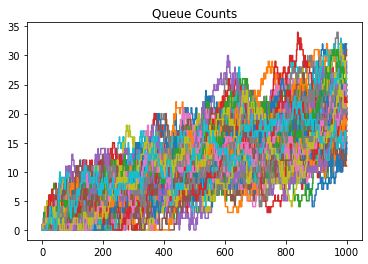
\includegraphics[scale=0.8]{redundancy}
    \caption{Plot using \lstinline{totals} of Figure~\ref{fig:red}}
    \label{fig:redpic}
\end{figure}

Remarkably, the simulation itself is performed speedily on consumer hardware despite the size of the system as demonstrated in Figure~\ref{fig:lstlisting2}.
\begin{figure}
    %! suppress = MissingLabel
    \begin{lstlisting}
CPU times: user 2.02 s, sys: 9.57 ms, total: 2.03 s
Wall time: 2.05 s
Intel i5-8250U (8) @ 3.400GHz
    \end{lstlisting}
    \centering
    \caption{Runtime Statistics}
    \label{fig:lstlisting2}
\end{figure}


Altogether, this makes the package easy to parallelize with and thus to compare systems of different sizes
and with large running-times.
While currently not implemented in any development branch of \textit{ParallelQueue}, the base Python package
\textit{multiprocessing} is used in throughout this paper when simulating for the same system across parameters.
In general, the main caveat when processing many models is that the storage of the simulation results can quickly begin
to consume storage;
when processing many models, therefore ensure that they are saved (e.g., using \textit{pickle}) and removed from
the local environment when doing analysis.

In terms of development, the models implemented in the \textit{base\_models} module use the framework established in~\ref{ch:model-specification}.
That is, modelling redundancy, a hyperedge of sorts is generated whence the dispatcher
receives a job to be cloned.
This hyperedge then exists for the duration of time for which the replica class is in the system and is defined in such
a way that \textit{Monitor} class objects can interact with them in order to acquire data.
In Python, such a data structure can be implemented rather easily by employing the \textit{Dict} type which defines
a keyed set of values.
By keying based on the job arrivals (before cloning), a unique set of marks can be retrieved for the set by simply using
the \textit{Dict} object as a reference.

\begin{figure}
    \centering
    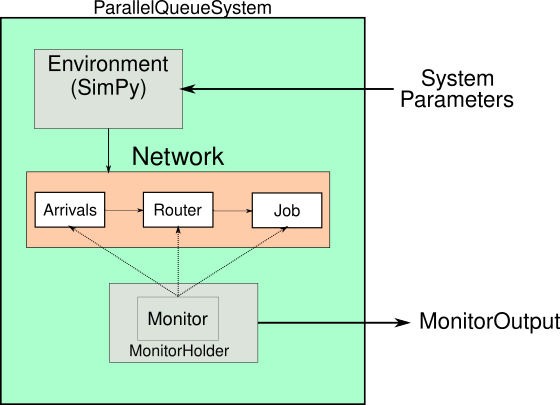
\includegraphics[scale=0.7]{pq}
    \caption{Overview of the ParallelQueue API}
    \label{fig:API}
\end{figure}


\section{Results}\label{sec:results}
First, we examine each model in terms of their respective performance in $E(T)$, the expected time each job spends in the system.
As Figure~\ref{fig:img} shows, for a load $\rho \triangleq \frac{\lambda}{\mu} = 0.5$ by taking $\mu=1, \lambda = 0.5$ (we will assume $\mu \equiv 1$ for the
rest of the simulations) , Redundancy(2)) and Threshold(2,2) policies are rather alike with low loads as $N \rightarrow \infty$. This is to be expected, of course, given that even such a low threshold is unlikely to be exceeded with the processors acting faster than arrivals on average. Ignoring cancellation costs, this clearly demonstrates how utilizing otherwise dormant queues comes to benefit the system's performance. Note that the figure is generated with the \textit{same} seed generation scheme for 30 different seeds per iteration, making the overlap a product of the two accessing random numbers from the system at the same points in time (in their respective simulations).

\begin{figure}
    \centering
    \includegraphics[width=0.7\linewidth]{} % [MISSING] - TODO: find this image + add to git
    \caption{Comparisons of Systems: Values are averaged over 30 independent iterations each, running for $t=1000$)}
    \label{fig:img}
\end{figure}

As~\cite{gardner_redundancy-d_2017} show, a Redundancy($d$) system is asymptotically stable if and only if $\rho < 1 $. Given that, in premise, Threshold($r,d$) models are more or less a superclass of Join-The-Shortest queue and Redundancy($d$) (trivially with rising $r$  implying no threshold exists and thus copies should always be made as in the case of Redundancy($d$), it is perhaps most interesting to examine if Threshold models are better able to handle high-load environments. Proving the superclass property in terms of Redundancy is relatively easy and is done in Lemma~\ref{sup}. By contrast, after merely setting $r \equiv 0$, we get $ \mathcal{D}_{\text{Thresh(0,d)}} \overset{d}{=} \mathcal{D}_{\text{JSQ(d)}}$ by definition.


\begin{lemma}
    \label{sup}
    For $\mathbf{X}^{(N)}$ being a system of queues such that $\rho < 1$, \[\mathcal{D}_{\text{Thresh(r,d)}}\mathbf(X^{(N)}) \overset{r \rightarrow \infty}{\rightsquigarrow} \mathcal{D}_{\text{Red(d)}}\mathbf(X^{(N)}).\]
\end{lemma}
\textit{Proof}:

Take $\leq_{st}$ to mean that~\cite{bramson_asymptotic_2012}
\[\mathbf{X}_{1}^{(N)}\leq_{st}\mathbf{X}_{2}^{(N)} \iff\# X_{1,i} \leq \# X_{2,i}  \quad \forall i \in [N] \quad P-a.s.\]
To show the sequence to be convergent, we will construct a coupling in such a manner that $\forall r \in \mathbb{R}^{+}$,  the system is bounded by another~\cite{baccelli_elements_2003} . For $\mathbf{X}_{1}^{(N)}$ under $\text{Thresh}(r,d)$, await the first arrival, denoted $T_{\xi_{1}}$, where a selection set, $\nu \subset [N] $ is prescribed such that $\exists \hat X \in \{X_{i}\}_{i \in \nu} $ such that $ \# (\hat X) > r $. Thus, for  $ t \in [0,T_{\xi_{1}})$, $\mathcal{D}_{\text{Thresh(r,d)}}\mathbf(X^{(n)}) = \mathcal{D}_{\text{Red(d)}}\mathbf(X^{(n)}) \quad$ . For clarity, let us now consider $\mathbf{Y}^{(N)}$ to be a copy of  $\mathbf{X}^{(N)}$ such that they are independent, identical in distribution and in terms of the marks of \textit{arrival process and job-size draws} along with the queues parsed (as was similarly done in~\cite{bramson_asymptotic_2012} Lemma 4.1); effectively, the only difference being left between these copies is $r$ changing which queues receive clones (and thus, too, the mark of queue-dependency).  $\mathcal{D}_{\text{Red(d)}}\mathbf(X^{(n)}) = \mathcal{D}_{\text{Thresh(r,d)}}\mathbf(Y^{(n)}) $; clearly, at time $T_{\xi_{1}}$, $\mathbf{X}^{(N)}\leq_{st}\mathbf{Y}^{(N)} $
due to jobs only being added for ${\hat Y_{i}}$ (defined analogously to  ${\hat X_{i}}$ ).

Now, assume $\rho< 1$, giving us $ \# Y_{i}  < \infty \quad \forall t \in \mathbb{R}^{+}$ with probability 1~\cite{gardner_redundancy-d_2017}. As such, we have that $\forall r \left[\exists \xi_{1}(r) | P_{r}\left(\mathbf{X}^{(N)} (t) = \mathbf{Y}^{(N)}(t) |t \in [0,T_{\xi_{1}}) \right) = 1\right]$ such that $\xi_{1} (r)$ is monotone increasing in $r$ and where $P_{r}(A) = P(\mathcal{D}_{M(r)}(A))$ for routing algorithm of $A$ being $M$. Letting $r \rightarrow \infty \Rightarrow \xi_{1} \rightarrow \infty$, we then have $\mathbf{X}^{(N)}(t) =  \mathbf{Y}^{(N)}(t) \quad \forall t \in \mathbb{R}^{+}$ in terms of distribution (i.e., as the result holds $\forall t \in \mathbb{R}^{+}$ as $r\rightarrow \infty$), implying the required weak convergence for $\mathcal{D}$ in law over system  $\mathbf{X}^{(N)}(t)$.  \qed

In order to evaluate the results of these simulations directly, the work of~\cite{campbell2020local} provides statistical notions of asymptotic exchangeability in the de Finetti sense by means of quantifying \textit{local} empirical measure sequences.

\begin{definition}[Local exchangeability]
    $\mathbb{X}$ is a locally exchangeable process if and only if there exists process $G_{t}$ where $\forall T \subset \mathbb{R}, \gamma \in \text(X,\Gamma) $
    \[P\left(\bigcap_{t \in T} \{X_{t} \in A\} | G^{(T)}_{t} \right) = \prod_{t \in T} G_{t} \quad \text{P-a.s.}\]
    \[\sup_{\omega}E|G^{(T)}_{t} (\omega)-G^{(T)}_{\gamma t}| \leq \sum_{t \in T} d(t, \gamma(t))\]

    where $G^{(T)}_{t}$ refers to $G_{t}$ restricted to $T$ and $d$ is a premetric which can be generated by means of finding the canonical premetric of the process.
\end{definition}
In essence, this is formulation provides a means of reducing time-exchangeability -- a problem concerning the probabilistic behaviour of a group-theoretic operator -- into a problem of analysis. While not necessarily implying exchangeability, local exchangeability provides a sufficient condition upon fulfilment of an additional criterion for full exchangeability: $d(t,t') \overset{|t-t'|\rightarrow 0}\rightarrow O(|t-t|^{1+a})$ for $a>1$.

In terms of $N \rightarrow \infty$, obviously it is important to consider $\rho$. For extremely low values of $\rho$, we expect the probability of the threshold being breached at a high $N$ at any time to approach zero. This is examined, for example, in Figure~\ref{fig:img1}. For this image, each value of $\rho$, $N \in \{2, 12, \dots 42\}$ is tested and prescribed a bar representing that $N \times \rho$ combination's $E(T)$ until $t=1000$ (each combination being run 30 times with independent seeds). Going forward, this suggests that we can examine rather high levels of $\rho$ to better contrast the difference between redundancy and non-redundancy models. Moreover, as we are evaluating the efficacy of this model for any $d$ choices, we place particular emphasis on $d \equiv 2$ given that returns from increasing $d$ tends to decrease regardless of whether replicas are or are not being considered~\cite{gardner_redundancy-d_2017,power}.
% TODO: \usepackage{graphicx} required
\begin{figure}
    \centering
    \includegraphics[width=0.7\linewidth]{} % [MISSING] - TODO: find this image + add to git
    \caption{Threshold(2,2) for Varying $N$ and $\rho$}
    \label{fig:img1}
\end{figure}

%\rho changed from what actually was \rho_{original} * d = 5 where 2 would be d
First, we look at Redundancy(2) under $\rho = 2.5$ for varying levels of $N$. Under the conjecture, we would expect convergence in $t$ whence the ECDFs over $t$ no longer change. As Figure~\ref{fig:redecdf} shows, this indeed seems to be the case when evaluating the ECDF at each time point wherein an event occurs for values up to 10 (which is never surpassed across the simulations). That is, a point mass at $0$ would indicate that the random variable seldom changes - a feat which seems to occur in this instance. To visualize the effect of then taking $t \rightarrow \infty$, let $\tilde{\tau}$ be the times at which an arrival or exit occurs (after the first arrival). Figure~\ref{fig:taus} can be produced by plotting histograms at different event times $\tilde{\tau}$.

\begin{figure}
    \centering
    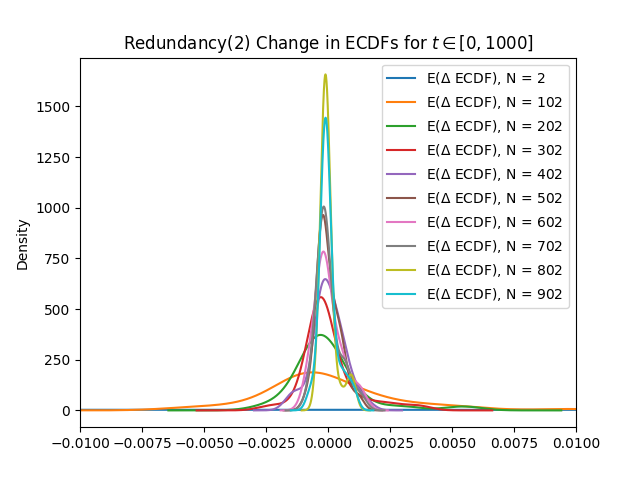
\includegraphics[width=0.7\linewidth]{redundancyecdf}
    \caption{Redundancy(2) ECDFs for Varying $N$}
    \label{fig:redecdf}
\end{figure}

\begin{figure}
    \centering
    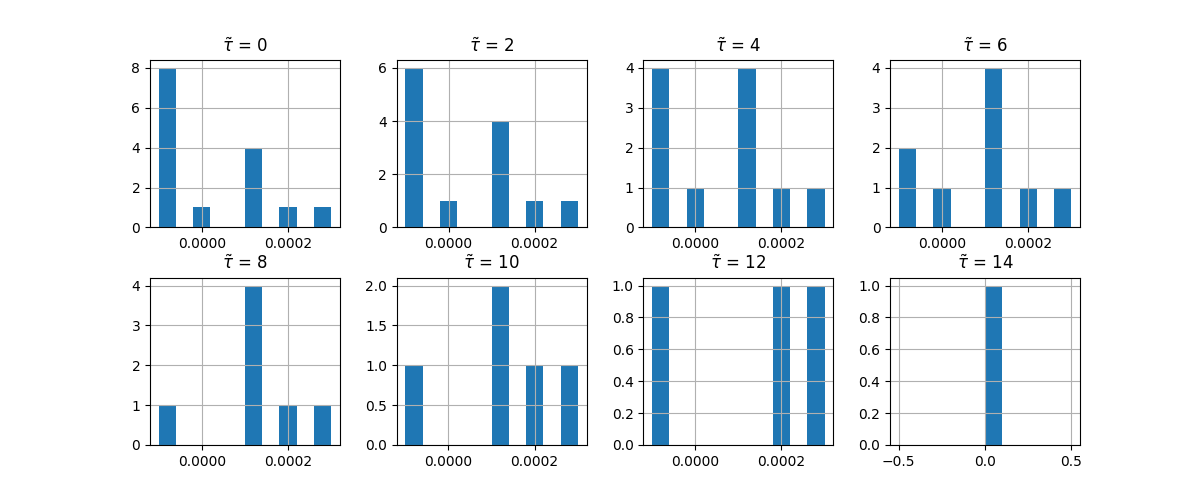
\includegraphics[width=0.8\linewidth]{redtau}
    \caption{Redundancy(2) Histograms of ECDF Changes for Varying $\tilde \tau$ at $N=1000$}
    \label{fig:taus}
\end{figure}


    %! Author = ajst
%! Date = 2021-02-28

% Preamble
\chapter{Concluding Remarks}\label{ch:discussion}

In all, with respect to the hypothesized behaviour specified in Conjecture~\ref{conj}, we were able to find support for asymptotic independence between queues in
$\mathbf{X}^{(N)}_{t}$ as $t\rightarrow \infty$ and $N\rightarrow \infty$, respectively at $r \in \{1,2\}, d = 2$.
Moreover, after iterating the limits, we found support for the system turning deterministic in law.
Along with the model developed for the system as outlined in Chapter~\ref{ch:model-specification}, a framework for formally proving the result in a manner similar to~\cite{bramson_asymptotic_2012}
is both introduced and demonstrated to likely be true for the tested parameters.

Outside of demonstrating the conjectured behaviour, this research has also highlighted some potentiallyinteresting directions
for future research into stochastic simulation and independence testing. 
With respect to simulations, \textit{ParallelQueue} was of course developed primarily for the systems studied in this paper.
While it was demonstrably fast in terms of single-process simulation, parallelizing in order to efficiently simulate multiple replications of the process
at once proved to be a memory-intensive task and necessitated porting the codebase into Cython.
This highlights the need for the development of a low-level DES framework which can efficiently manage memory and resources between simultaneous simulations of a process.

In terms of independence testing, this research has demonstrated the need for further exploration into methods for discrete processes and group independence.
Clearly, for a queueing process which does not ``explode'', we would expect that queue counts do not increase indefinitely~\cite{gardner_redundancy-d_2017}.
In our tests, such seems to have left queues with relatively little variance to study (in most cases, queue counts were binary for $N>5$), perhaps biasing results against the null hypothesis.
Lastly, with respect to group dependence, the fact that a counting process would have only been able to depend on a maximum of $d-1$ others could perhaps have been utilized when determining a statistic for group independence
across time samples.
Future research in independence testing, especially with respect to $d$HSIC/HSIC, might therefore benefit from exploring bootstrap estimators for constrained groupings.




%----------------------------------------------------------------------
% END MATERIAL
% Bibliography, Appendices, Index, etc.
%----------------------------------------------------------------------

% Bibliography

% The following statement selects the style to use for references.  It controls the sort order of the entries in the bibliography and also the formatting for the in-text labels.
\bibliographystyle{ieeetr}
% This specifies the location of the file containing the bibliographic information.
% It assumes you're using BibTeX to manage your references (if not, why not?).
    \cleardoublepage % This is needed if the book class is used, to place the anchor in the correct page,
    % because the bibliography will start on its own page.
    % Use \clearpage instead if the document class uses the "oneside" argument
    \phantomsection  % With hyperref package, enables hyperlinking from the table of contents to bibliography
% The following statement causes the title "References" to be used for the bibliography section:
    \renewcommand*{\bibname}{References}

% Add the References to the Table of Contents
    \addcontentsline{toc}{chapter}{\textbf{References}}

    \bibliography{main}
% Tip 5: You can create multiple .bib files to organize your references.
% Just list them all in the \bibliogaphy command, separated by commas (no spaces).

% The following statement causes the specified references to be added to the bibliography% even if they were not
% cited in the text. The asterisk is a wildcard that causes all entries in the bibliographic database to be included (optional).\nocite{*}
%----------------------------------------------------------------------

% Appendices
% The \appendix statement indicates the beginning of the appendices.
    \begin{appendices}
        %! Author = ajst
%! Date = 2021-02-26

\chapter{$d$HSIC Resampling Cython Implementation}\label{sec:sic}

\begin{lstlisting}[label={lst:cyhsic}, language=Cython, style=mystyle]
#cython: language_level=3
#cython: infer_types=True
import random
from copy import deepcopy
import numpy as np
cimport numpy as np
from sklearn.metrics import pairwise_distances
from sklearn.metrics import pairwise_kernels

cpdef width(Z):
    dist_mat = pairwise_distances(Z, metric='euclidean')
    return np.median(dist_mat[dist_mat > 0])

cdef center_k(X, width_X, m=None):
    if m is None:
        m = X.shape[0]
    H = np.eye(m) - (1 / m) * (np.ones((m, m)))
    K = pairwise_kernels(X, X, metric='rbf', gamma=0.5 / (width_X ** 2))
    K = H @ K @ H
    return K

cpdef list time_sampler(X, time_samples, max_time = 1000):
    """
    For a list of runs of the same process, returns array of each at specified times.
    Samples using binary search algorithm (https://numpy.org/doc/stable/reference/generated/numpy.searchsorted.html).
    
    :param X: list of time-indexed (sorted) data of the same process with the same max running time.
    :param time_samples: list of times to sample at.
    :param max_time: maximum allotted time per simulation.
    :return: data at sampled times.
    """
    cdef list ret = []
    for time in time_samples:
        data_slice = []
        for proc in X:
            time_list = list(proc.keys())
            insertion_point = np.searchsorted(time_list, time)  # a[i-1] < v <= a[i] via binary search algo
            if time_list[insertion_point] != time:
                insertion_point = time_list[insertion_point - 1]  # Cadlag
            data_slice.append(proc[insertion_point])
        ret.append(data_slice)
    return ret

cdef dHSIC_hat(Xs):
    """https://arxiv.org/pdf/1603.00285.pdf -- see algorithm 1"""
    cdef int x_len = Xs[0].shape[0]
    #inits
    t1 = 1
    t2 = 1
    t3 = (2 / x_len)
    for x in Xs:
        K = center_k(x, width(x))
        t1 = np.multiply(t1, K)
        t2 = (1 / x_len ** 2) * t2 * np.sum(K)
        t3 = (1 / x_len) * t3 + np.sum(K, axis=0)
    return (1 / x_len ** 2) * np.sum(t1) + t2 - np.sum(t3)

cpdef dHSIC_resample_test(list Xs, int shuffle=500, float alpha = 0.05):
    """Resampling implementation -- see sec 4.3. of https://arxiv.org/pdf/1603.00285.pdf
     Returns stat and threshold (if possible)."""
    init = dHSIC_hat(Xs)
    locX = deepcopy(Xs) # deep copy
    cdef int hits = 0
    cdef list dXs = []
    for i in range(shuffle):
        random.shuffle(locX)  # void shuffles
        permed = dHSIC_hat(locX)
        if permed >= init:
            hits += 1
        dXs.append(permed)
    dXs.sort()
    critIndex = 0
    for i in range(shuffle):
        if dXs[i] == init:
            critIndex += 1
    critIndex += np.ceil((1-alpha) * (shuffle + 1))
    critIndex = int(critIndex)
    if critIndex < shuffle:
        thrsh = dXs[critIndex]
    else:
        thrsh = None
    #stat, threshold
    return (hits + 1) / (shuffle + 1), thrsh
\end{lstlisting}


    \end{appendices}
% Add a title page before the appendices and a line in the Table of Contents
% Appendices are just more chapters, with different labeling.

%----------------------------------------------------------------------
\end{document} % end of logical document
